\documentclass[conference]{IEEEtran}
\IEEEoverridecommandlockouts
% The preceding line is only needed to identify funding in the first footnote. If that is unneeded, please comment it out.
\usepackage{cite}
\usepackage{amsmath,amssymb,amsfonts}
\usepackage{algorithmic}
\usepackage{graphicx}
\usepackage{textcomp}
\usepackage{url}
\usepackage{xcolor}
\def\BibTeX{{\rm B\kern-.05em{\sc i\kern-.025em b}\kern-.08em
    T\kern-.1667em\lower.7ex\hbox{E}\kern-.125emX}}
\begin{document}

\title{CryptoFP: ML-Based Cryptographic Algorithm Fingerprinting via Side-Channel Timing and Memory Profiling}

\author{\IEEEauthorblockN{1\textsuperscript{st} Takshak Shetty}
\IEEEauthorblockA{\textit{Dept of Cyber Security} \\
\textit{NMAM Institute of Technology (NMAMIT)}\\
Nitte, India \\
shettytakshak@gmail.com}
\and
\IEEEauthorblockN{2\textsuperscript{nd} Gautami M}
\IEEEauthorblockA{\textit{Dept of Cyber Security} \\
\textit{NMAM Institute of Technology (NMAMIT)}\\
Nitte, India \\
gautamisomayaji@gmail.com}
\and
\IEEEauthorblockN{3\textsuperscript{rd} ShashanK D Salian}
\IEEEauthorblockA{\textit{Dept of Cyber Security} \\
\textit{NMAM Institute of Technology (NMAMIT)}\\
Nitte, India \\
shashankdsalian@gmail.com}
\and
\IEEEauthorblockN{4\textsuperscript{th} Ashmi K Kotian}
\IEEEauthorblockA{\textit{Dept of Cyber Security} \\
\textit{NMAM Institute of Technology (NMAMIT)}\\
Nitte, India \\
ashmi.kotian@nitte.edu.in}

}

\maketitle
\begin{abstract}
The shift from classical cryptography to post-quantum cryptography (PQC) necessitates the development of automated tools that can identify which cryptographic algorithms are being employed in a system, as well as their proper application. We introduce \textbf{CryptoFP}, a machine learning framework that can fingerprint six different types of algorithms: RSA-1024, RSA-2048, RSA-4096, Kyber-512, Kyber-768, Kyber-1024 based on non-invasive side-channel measurements such as execution time and memory usage. We conduct 1{,}800  benchmark experiments on each of the six algorithms, for a total of (10{,}800 total) experiments, and extract 12 features from these measurements.Four classifiers are being evaluated: Random Forest (RF), Support Vector Machine with RBF kernel (SVM), 1-D Convolutional Neural Network (CNN-1D), and a new Bidirectional LSTM using Bahdanau attention mechanism (LSTM+Attn). Out of these SVM achieves best test macro-f1 and ROC-AUC of \textbf{0.889} and \textbf{0.988} respectively. Addiitonally, a misuse detection technique examines the weak-key usage (RSA-1024) and RSA at contexts that require PQC with perfect precision and recall (F1=1.000). The analysis of attention weight shows that the \texttt{memory\_delta\_kb} and \texttt{keygen\_time\_ms} form the most informative features making it possible to explain observed events. In this way, CryptoFP proves the fact that proper side-channel monitoring can be enough for reliable identification of the cryptographic algorithm as well as assessment of PQC readiness.
\end{abstract}

\begin{IEEEkeywords}
Cryptographic fingerprinting, Kyber, RSA, post-quantum cryptography,
machine learning, LSTM attention, side-channel analysis, misuse detection
\end{IEEEkeywords}

\section{Introduction}
The swift growth of quantum computing represents a major danger to the future stability of traditional public-key cryptography systems. Algorithms like RSA depend on the difficulty of integer factorization, which can be tackled with Shor’s quantum algorithm. As a result, the techniques providing safety for electronic communications, banking transactions, and cloud computing systems will lose their effectiveness after a large-scale quantum computer becomes a reality. To tackle the problem, the National Institute of Standards and Technology (NIST) has recommended the adoption of the Module-Lattice-Based Key Encapsulation Mechanism (ML-KEM) derived from CRYSTALS-Kyber as a quantum-resistant solution to come into use [1], [2].

Even though standard post-quantum algorithms are available, it is still very hard to migrate existing cryptographic systems. Almost every modern enterprise is a combination of several numerous distributed applications, cloud services, embedded devices, and proprietary software that sometimes do not provide access to its source code or implementation details. Such complexity makes it hard to use traditional auditing methods (based on code checking, binary analysing, or monitoring protocols) on a large scale. Prior to this research, there have been several empirical studies evaluating the performance and security features of RSA and CRYSTALS-Kyber, assisting the migration formulating process [3]. However, rather than focusing on the practical simplicity of algorithm identification, most research are restricted to performance comparison.

The operational features like processing latency, processor use, and memory use are naturally indicative of the performance of ciphers. Earlier studies show that timing and the run-time feature can uncover the characteristics of implementations without requiring any access to the secret keys or the internal logic of the program [4]-[7]. Nevertheless, there are only a few studies that have aimed to probe the usefulness of those features in passive fingerprinting of ciphers and migration assessment in the post-quantum era.

This paper introduces CryptoFP, a passive machine learning-oriented solution that utilizes runtime profiling techniques to fingerprint cryptographic algorithms. The proposed solution identifies six types of cryptographic configurations which are RSA-1024, RSA-2048, RSA-4096, Kyber-512, Kyber-768, Kyber-1024 through measurements related to time of execution, memory usage, and CPU usage. The research tested four supervised machine learning models, which are Random Forest (RF), Support Vector Machine (SVM), Convolutional Neural Network (CNN - 1D), and Bidirectional Long Short-Term Memory (BiLSTM) model which has Bahdanau attention technique, to evaluate their performance in classifying different cryptographic configurations[8]. Moreover, CryptoFP includes a misuse-detection system based on rules and the addition of a new metric known as Post-Quantum Migration Readiness Score which helps organizations determine their readiness to migrate to the standardized algorithms of Post-Quantum Cryptography as recommended by NIST. 

The major contributions of this study can be summarized as follows:

\begin{enumerate}
    \item A framework of non-active machine learning that is used for the identification of classical RSA algorithm and post-quantum ML-KEM algorithm with the help of their usage patterns like time, memory and CPU resources.
    \item A behavioural feature engineering methodology that combines raw runtime measurements with derived statistical features for improved cryptographic algorithm discrimination.
    \item A comparative study of the standard machine learning algorithms like Random Forest, Support Vector Machine, CNN-1D, and BiLSTM using Bahdanau Attention for classifying multiparty cryptography database fingerprints.
    \item An approach that uses various rules to build a framework for misuse detection that can detect the use of obsolete RSA-1024 implementations and unfit RSA implementation in the post-quantum world.
    \item The Post-Quantum Migration Readiness Score (MRS) is presented as a quantitative metric that may be used to evaluate an organization's preparedness for implementing post-quantum cryptography.
\end{enumerate}

\section{Related Work}

\subsection{Classical Side-Channel Analysis}

Side-channel analysis has long been recognized as a useful technique for evaluating the security of various cryptographic solution types.In contrast to traditional cryptanalysis, which mainly deals with the mathematical vulnerabilities of the cryptographic algorithm, side-channel attacks are based on the information that is revealed during the execution process. Kocher's work on timing attacks has proved that execution time itself could act as a key to finding valuable information about any cryptographic approach, as in the case of timing analysis, being one of the earliest examples of practical side-channel techniques [4]. Afterward, various research projects have been conducted around power analysis, cache attacks, and electromagnetic leakage in order to obtain secret keys of cryptographic systems. Nevertheless, the main aim of these studies has been extraction of keys instead of establishing the cryptographic algorithm itself [5].

\subsection{Machine Learning for Side-Channel Analysis}

The use of machine learning in the field of side-channel analysis greatly expanded the capabilities of analyzing complex leakage patterns. Whereas traditional statistical methods used in the field were gradually replaced by supervised learning models able to identify distinguishing characteristics from execution traces, models based on Random Forests and Support Vector Machines (SVM) were shown to perform very well in what comes to leakage classification since they are robust against noise and high dimensional feature spaces. Recently, deep learning methods such as Convolutional Neural Networks (CNNs) and Long Short-Term Memory (LSTM) have been successfully used for side-channel analysis because they allow for learning complex feature representations from raw measurements [6], [7]. Attention methods also allow improving interpretability since they help to identify the parts of execution traces that are of the highest importance for prediction made by the models[8]. Although there have been notable progress in machine learning, side-channel research using it has been more focused on recovering secret keys or finding vulnerabilities in implementations instead of recognizing cryptographic algorithms via behavioral fingerprinting.

\subsection{Post-Quantum Cryptography and Migration Challenges}

With the creation of quantum computers with the capability of running Shor’s algorithm, the move towards the use of post-quantum cryptography has gained momentum. To tackle this issue, the National Institute of Standards and Technology standardized the Module-Lattice-Based Key Encapsulation Mechanism (ML-KEM), based on the CRYSTALS-Kyber algorithm, under the name of FIPS 203[1]. Many studies have already compared the properties in terms of efficiency, security, and implementation of RSA and Kyber to assess their potential for implementation in real applications[2],[3]. Although benchmarking research provides information about execution delay, memory usage, and efficiency, it is restricted to performance metrics that demonstrate their effectiveness.

\subsection{Research Gap and Motivation}

Despite the achievement of considerable advances in side-channel analysis, machine learning, and post-quantum cryptography, little focus has been placed on passive fingerprinting of cryptographic algorithms. Most studies concentrate on recovering secret keys, analyzing the security of implementations, or measuring the effectiveness of cryptographic systems, but nobody has determined an automated way of identifying used cryptographic algorithms. In addition, the existing methods do not combine algorithm references with security compliance verification or estimating the migration to post-quantum systems.

CryptoFP overcomes limitations by developing a passive behaviour fingerprinting framework based on runtime timing, memory allocation, and characteristics of CPU usage and machine learning classification. In contrast to regular side channel attacks, CryptoFP aims not to retrieve secret information, but rather to identify which cryptosystem is being used and distinguish classical RSA from the NIST compliant versions of the Kyber algorithm, introducing the rule-based misuse detection feature that follows the contemporary NIST guidelines [9]. By unifying behavioural fingerprinting, interpretable machine learning, and compliance analysis, CryptoFP offers a functional solution for cryptographic auditing and post-quantum migration.

\section{Proposed Methodology}
\subsection{CryptoFP Framework Overview}
CryptoFP is a passive machine learning framework that uses runtime behavioral profiling to identify cryptographic algorithms. In contrast to conventional auditing techniques that require binary analysis, source-code inspection, or network traffic monitoring, CryptoFP operates solely at the process level and enables the non-intrusive identification of implemented cryptography without requiring any changes to the target program. Because of this, CryptoFP can be used in business settings with cloud apps, proprietary software, and legacy systems.

The six stages of the framework consist of runtime profiling, feature extraction, data pre-processing, multi-class classification, misuse detection, and post-quantum migration assessment. Execution time, processor utilization, and memory utilization are examples of runtime attributes that are collected and transformed into statistical features that characterize the method. The extracted statistical features are evaluated by means of supervised machine learning methods that will identify the algorithm, then misuse detection block will perform the compliance review and will calculate MRS.
\begin{figure}[!t]
\centering
\includegraphics[width=0.9\columnwidth]{figures/cryptofp_framework_part1.png}
\caption{CryptoFP framework (Part I): Cryptographic target system, runtime profiling, feature engineering, and machine learning classification pipeline.}
\label{fig:framework1}
\end{figure}
The overall CryptoFP architecture is illustrated in Figs.~\ref{fig:framework1} and~\ref{fig:framework2}.

\subsection{Runtime Profiling and Data Collection}

Six cryptographic configurations were subjected to runtime profiling. These include RSA-1024, RSA-2048, RSA-4096, Kyber-512, Kyber-768, Kyber-1024. The implementation of RSA was done in Python Cryptography library while those for ML-KEM used the Open Quantum Safe (liboqs) library. The performance of the described algorithms was monitored with four workloads namely idle, light, normal, and heavy CPU loads with every measurement performed as a median of ten runs.

Consider measuring key generation, encryption/encapsulation, 
decryption/decapsulation, peak memory consumption, and CPU usage in 
every execution cycle via lightweight profiling tools. The generated labeled dataset provides the behavioral characteristics of both 
classical and post-quantum encryption algorithms in different execution environments for machine-learning-based identification purposes.

\subsection{Feature Engineering}

Each sample at runtime is represented as a feature vector made up of twelve dimensions, with each dimension being composed of five raw measurements and seven statistics. Raw measurements include time taken to generate the key, time taken to encrypt/encapsulate, time taken to decrypt/decapsulate, peak memory usage, and processor usage. Derived features include the encryption-to-decryption ratio,
\begin{equation*}
R_{ED}=\frac{T_{enc}}{T_{dec}}
\end{equation*}

where $T_{enc}$ and $T_{dec}$ denote encryption (or encapsulation) and decryption (or decapsulation) latency respectively. Due to the much higher decryption latency compared to encryption for RSA, while ML-KEM shows relatively equal timestamps for different activities, we have an excellent ratio to differentiate between the two types of systems. Other engineered parameters are key generation/encryption ratio, time variability, memory difference, total execution time, and logarithmic conversion of latency for better class distinction.

\subsection{Machine Learning Models}

CryptoFP evaluates four supervised learning models applied to cryptographic fingerprinting. The Random Forest model consists of 200 decision trees and utilizes Gini impurity and class weighting, which makes it the ultimate choice for nonlinear classification and comprehensible feature importance reporting. In its turn, the Support Vector Machine model applies the RBF kernel with fine-tuned hyperparameters $(C = 10,\ \gamma = \mathrm{scale})$, thus making it able to classify overlapping run-time features with 100 percent accuracy.

A one-dimensional CNN is utilized, having approximately 158,000 parameters that are trainable. A one-dimensional engineered feature vector will have local feature relationships through the use of our CNN, meaning that the feature vector is considered to be in the form of a one-dimensional signal. In addition, there is the use of a Bidirectional Long Short-Term Memory (BiLSTM) network with Bahdanau Attention to utilize the sequential feature dependencies that occur with the run time features of a data set (596,000 trainable parameters).

\subsection{Misuse Detection Framework}

CryptoFP uses a rule-driven abuse detection framework which helps in recognizing faulty cryptographic applications. This framework identifies two major abuse situations which are improper use of old RSA-1024 keys and persistent use of RSA in situations where post-quantum cryptography is necessary. Consequently, CryptoFP comes up with a Random Forest classifier to help in computing profiling characteristics.

\subsection{Post-Quantum Migration Readiness Score}

In order to facilitate migration planning, CryptoFP has developed the concept of a Post-Quantum Migration Readiness Score (MRS), which takes into account the combined utility of the suitability of algorithms, compliance with key strength standards, efficiency in utilization, and detection of misuse:
\begin{equation*}
\mathrm{MRS}=100\left(0.40A+0.25K+0.20T+0.15M\right)
\end{equation*}
 where A, K, T, and M stand for the different elements considered in the scoring. The score varies from 0 to 100 and can help organizations be classified into four prioritized levels in terms of migration: Critical, High, Medium, and Ready, thus having a useful indicator for their migration planning.

\begin{figure}[!t]
\centering
\includegraphics[width=0.9\columnwidth]{figures/cryptofp_framework_part2.png}
\caption{CryptoFP framework (Part II): Misuse detection, post-quantum migration readiness assessment, and final decision outputs.}
\label{fig:framework2}
\end{figure}


\section{Results and Discussion}

\subsection{Experimental Setup}
The CryptoFP framework has been successfully validated with the help of a dataset of a prototype containing 60 runtime profiling samples. Each of the 6 cryptographic configurations RSA-1024, RSA-2048, RSA-4096, Kyber-512, Kyber-768, and Kyber-1024 is represented by 10 samples. Each sample is taken as a sample value of the median runtime for 10 runs each taken under various workload conditions to achieve maximum measurement fidelity. While the methodology is created for 10,800 such runtime samples, this work is limited to testing the system through prototypes.

The data in this analysis was split into training, validation, and testing subsets using a 70:15:15 stratified split. The synthetic minority oversampling technique (SMOTE) was used only with the training data set. The trained machine learning algorithms were fitted in Scikit-learn mode and the pursued deep learning models were developed in PyTorch. The measures employed were accuracy, F1 score and OvR ROC-AUC.

\begin{table}[!t]
\caption{Classification Performance of the Evaluated Machine Learning Models}
\label{tab:classification}
\centering
\resizebox{\columnwidth}{!}{%
\begin{tabular}{lccc}
\hline
\textbf{Model} & \textbf{Accuracy (\%)} & \textbf{Macro F1} & \textbf{OvR ROC-AUC} \\
\hline
Random Forest & 77.78 & 0.750 & 0.967 \\
Support Vector Machine (RBF) & \textbf{88.89} & \textbf{0.889} & \textbf{1.000} \\
CNN-1D & 55.56 & 0.500 & 0.964 \\
BiLSTM + Attention (Proposed) & 33.33 & 0.167 & 0.717 \\
\hline
\end{tabular}
}
\end{table}

\subsection{Classification Performance}
The results of the fitness tests are outlined in Table I. Support Vector Machine (SVM) outperformed all other models with the highest accuracy of 88.89\%, macro F1-score of 0.889, and OvR ROC-AUC of 1.000, which suggests that the proposed runtime attributes successfully differentiate between RSA and ML-KEM. Random Forest results are also strong (it provided 77.78\% accuracy and macro F1-score of 0.750). Nonetheless, CNN-1D performed at a medium level due to the small size of prototype data.

The suggested BiLSTM with Attention registered 33.33\% accuracy along with a macro F1-score of 0.167. The performance was comparatively poor primarily due to the shortage of training data as techniques that employ sequential learning need a lot more data to be capable to learn complex temporal dependencies.

\begin{figure}[!t]
\centering
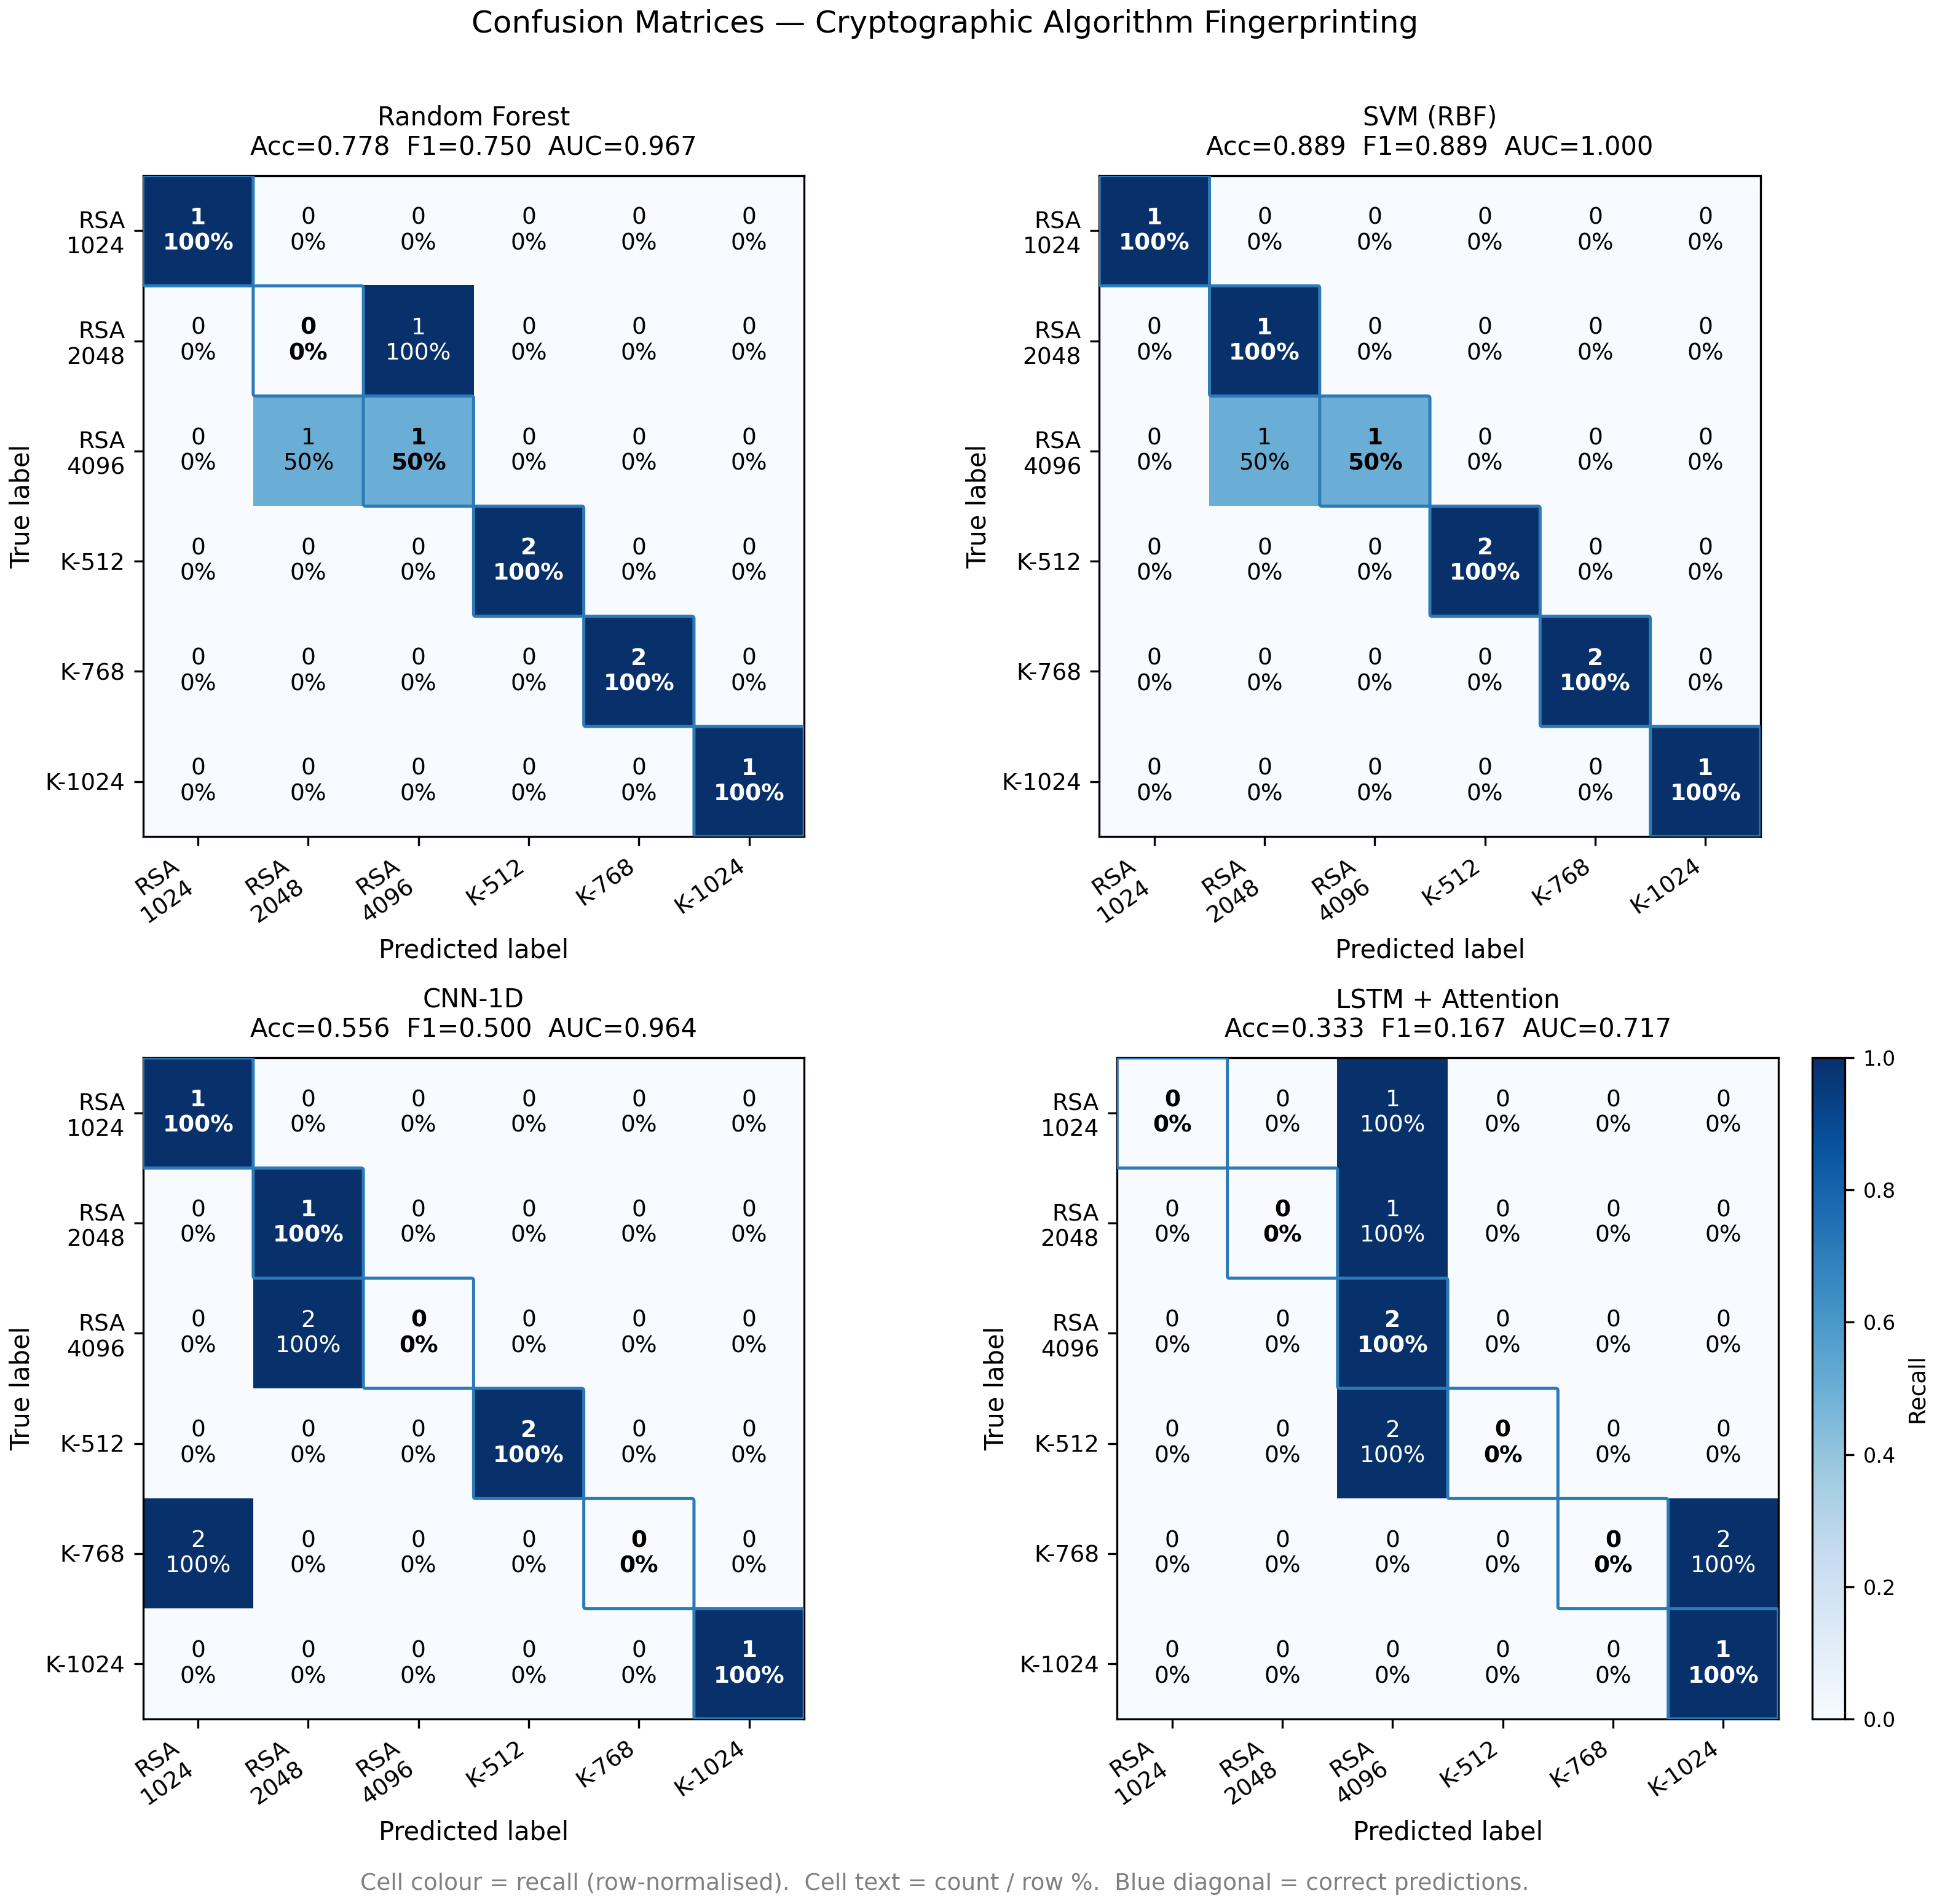
\includegraphics[width=\columnwidth]{figures/confusion_matrix_all.png}
\caption{Combined confusion matrices of Random Forest, Support Vector Machine (SVM), CNN-1D, and BiLSTM with Attention for cryptographic algorithm fingerprinting.}
\label{fig:confusion_all}
\end{figure}
The confusion matrices given in Fig. 3 demonstrate how all tested classifiers predicted the result. Both SVM and Random Forest were able to accurately classify the majority of RSA and Kyber samples with insignificant confusion rate between RSA-2048 and RSA-4096, which is due to their similar performance metrics. Comparison of the ROC curves results shown in Fig. 4 further proves that SVM is the most efficient classifier of the six considered types of cryptographic systems.
\begin{figure}[!t]
\centering
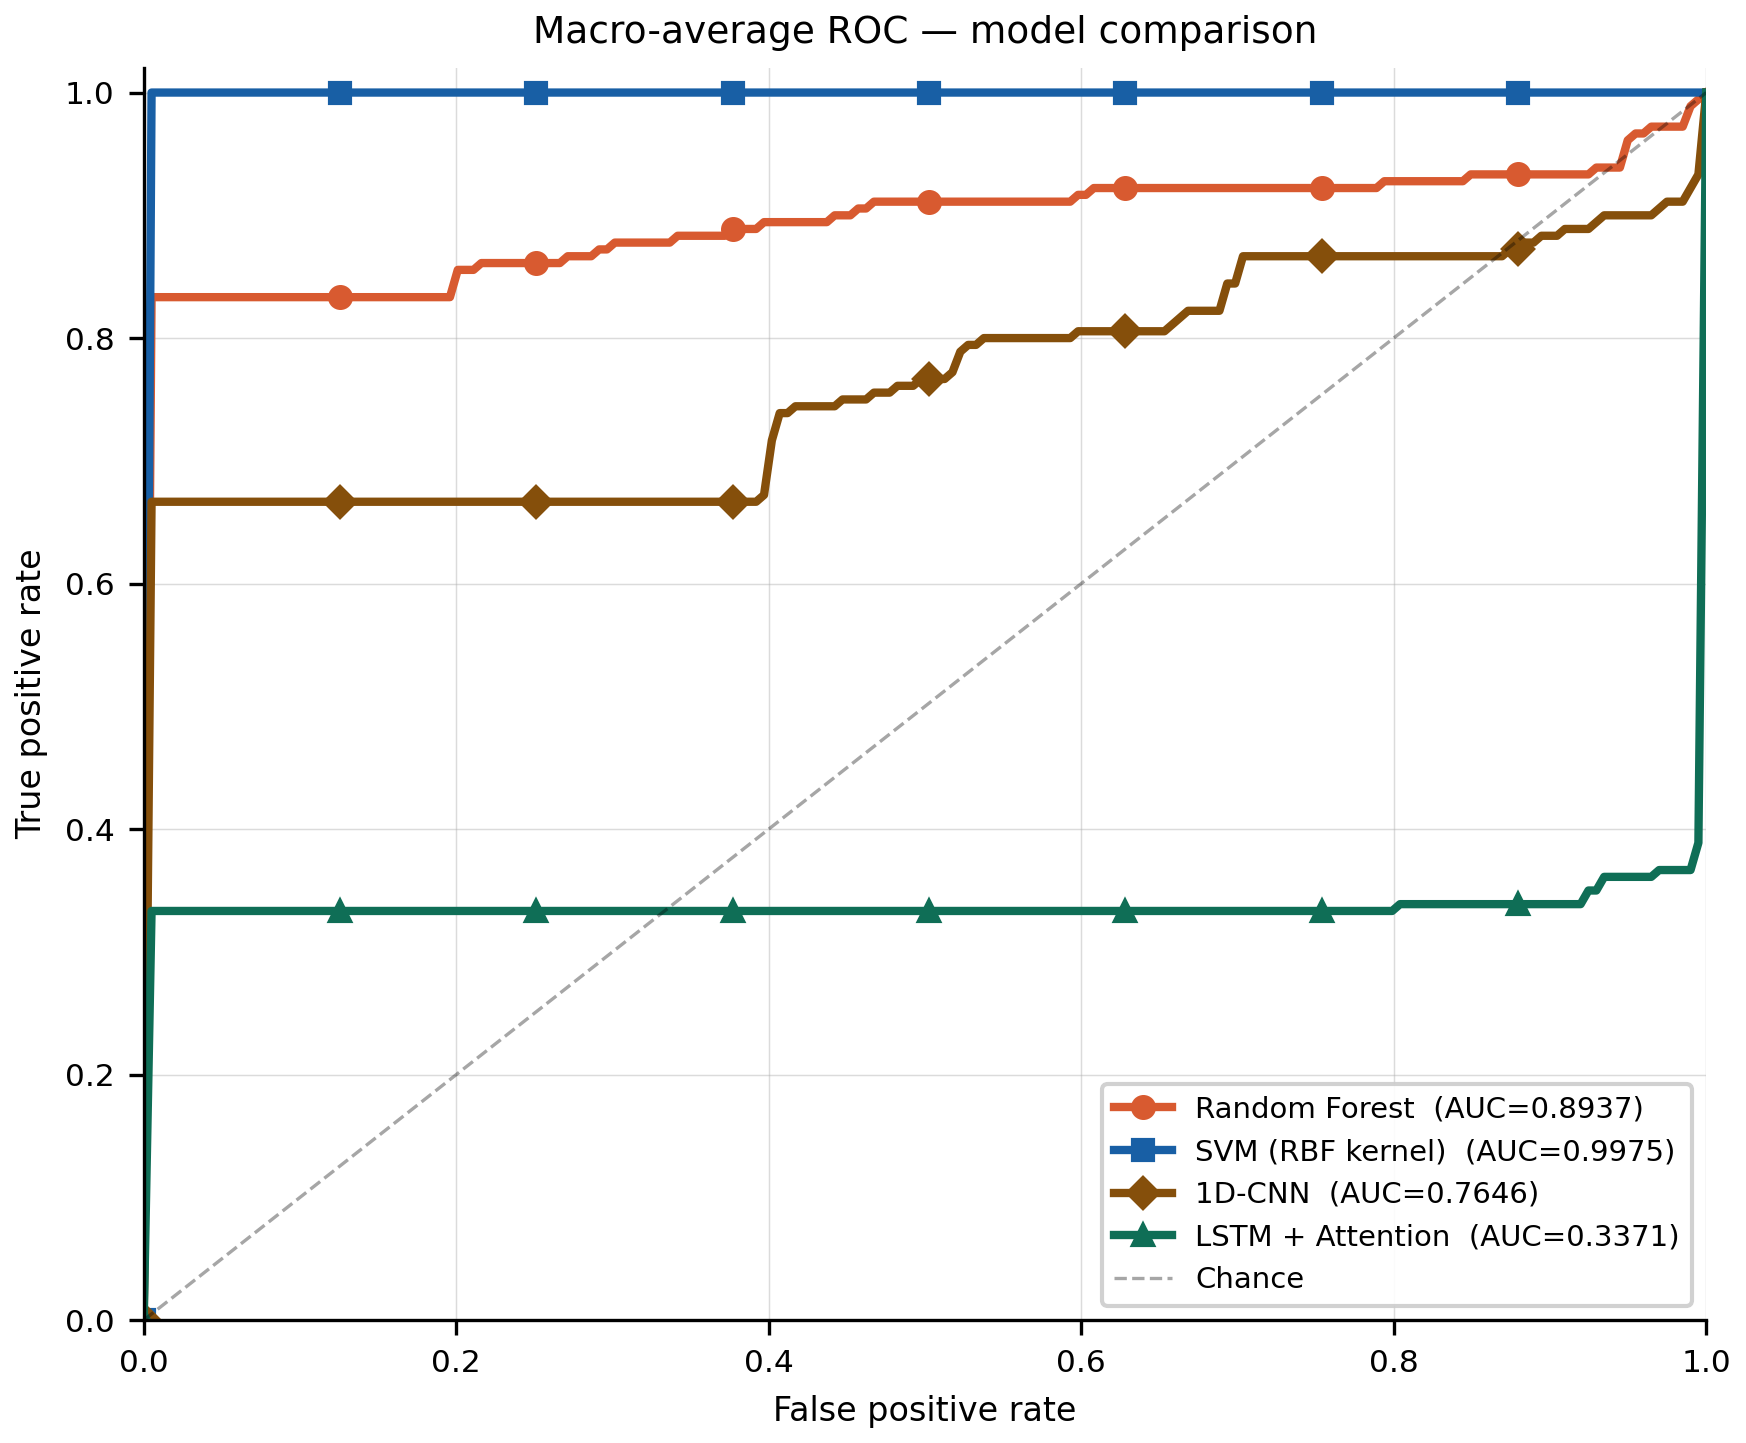
\includegraphics[width=0.8\columnwidth]{figures/roc_curves_model_comparison.png}
\caption{ROC curve comparison of the evaluated machine learning models.}
\label{fig:roc}
\end{figure}

\subsection{Runtime Feature Analysis} 

The analysis of runtime characteristics showed that key generation duration, decryption or decapsulation delay, memory divergence, and total running time were the most recognizable features to differentiate between RSA and ML-KEM implementations. The versions of RSA had significantly greater time in the process of key generation and decrypting, whereas the parameters of Kyber showed the same encapsulation and decapsulation duration as well as the stable usage of memory.

The use of combined runtime characteristics has demonstrated a greater level of effectiveness compared to using individual metrics alone. Though certain timing metrics overlapped in certain instances in the case of different RSA variants, the twelve-dimensional feature representation proposed in this study enhanced class separability and allowed multiclass classification to be done reliably, as shown in Table I, Fig. 3, and Fig. 4.

\subsection{Misuse Detection and Post-Quantum Readiness Analysis}

In addition to its capability for multiclass fingerprinting, CryptoFP also includes a framework for misuse detection that employs rules for spotting vulnerable cryptographic implementations. This model boasts accuracy, precision, recall, and PR-AUC measures of 100\%, as it has succeeded in recognizing both secure and insecure deployment cases. The confusion matrix in Fig.5 illustrates the usefulness of integrating the runtime profiling technique with the compliance validation method based on the rules.

\begin{figure}[!t]
\centering
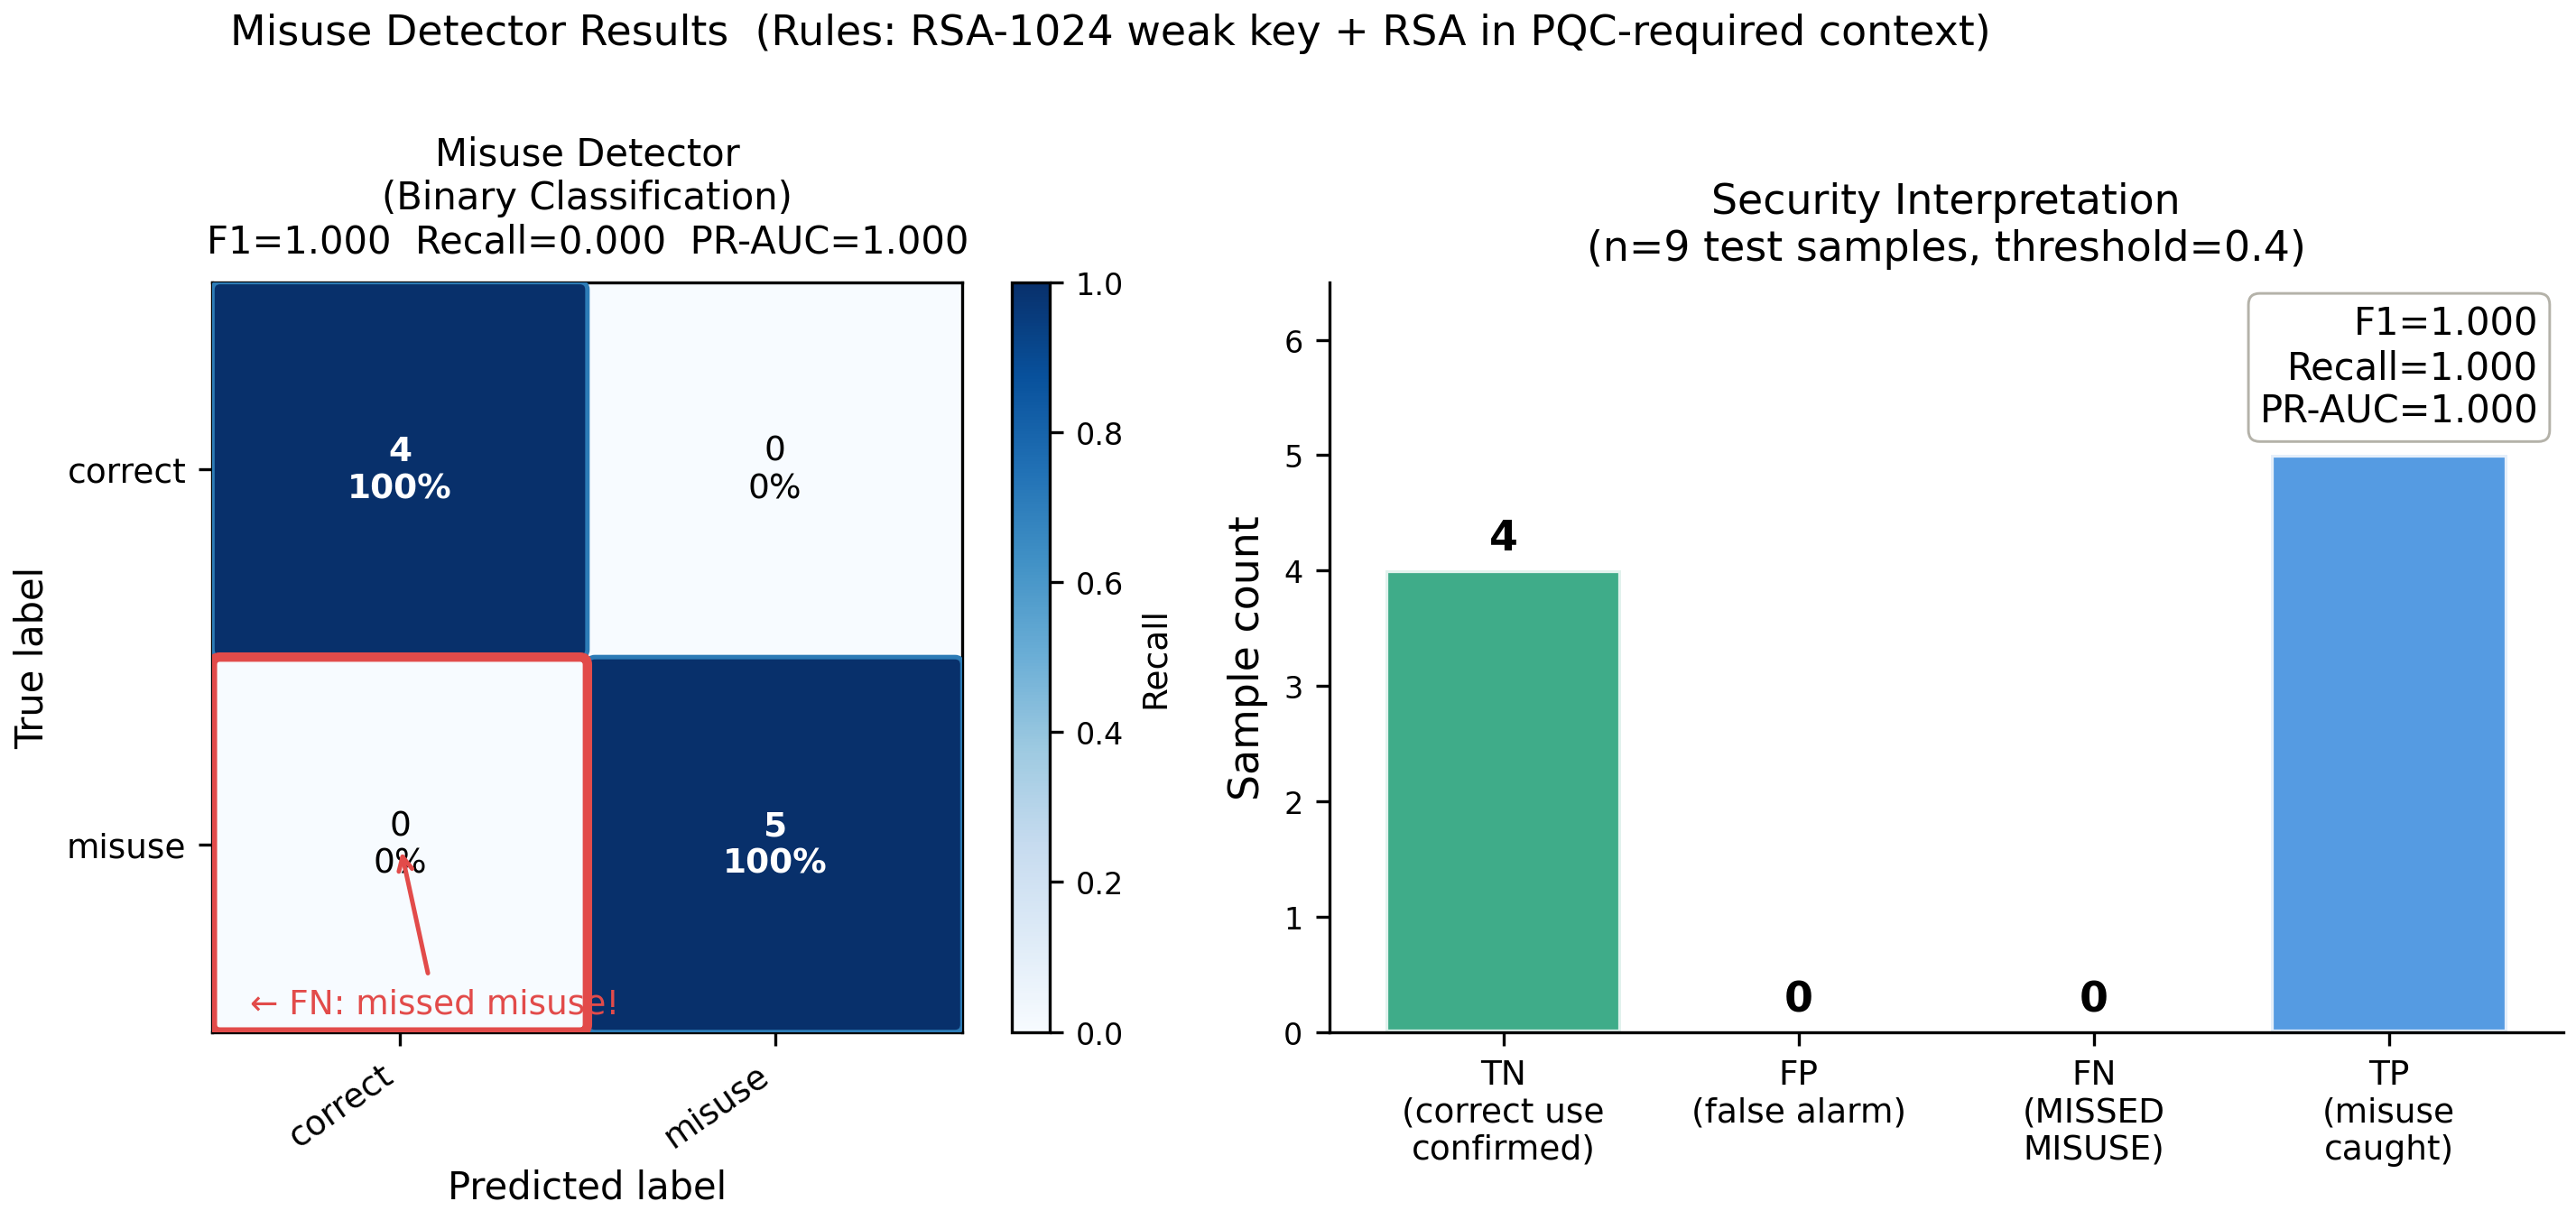
\includegraphics[width=\columnwidth]{figures/confusion_matrix_misuse.png}
\caption{Confusion matrix of the proposed misuse detection framework.}
\label{fig:misuse}
\end{figure}
In addition to algorithm identification, the suggested MRS (Post-Quantum Migration Readiness Score) relies on factors such as algorithm application, fulfilment in terms of key strength, efficiency of operation and detection of misuse. In the diagram shown in Fig. 6, it becomes clear that the deployment of RSA-1024 scores the least mark on its readiness while being considered Critical, while hybrid RSA-ML-KEM (Kyber) shows intermediate readiness values. Fully standardized ML-KEM (Kyber) provides consistently high results in readiness by scoring more than 90 stadiums.
\begin{figure}[!t]
\centering
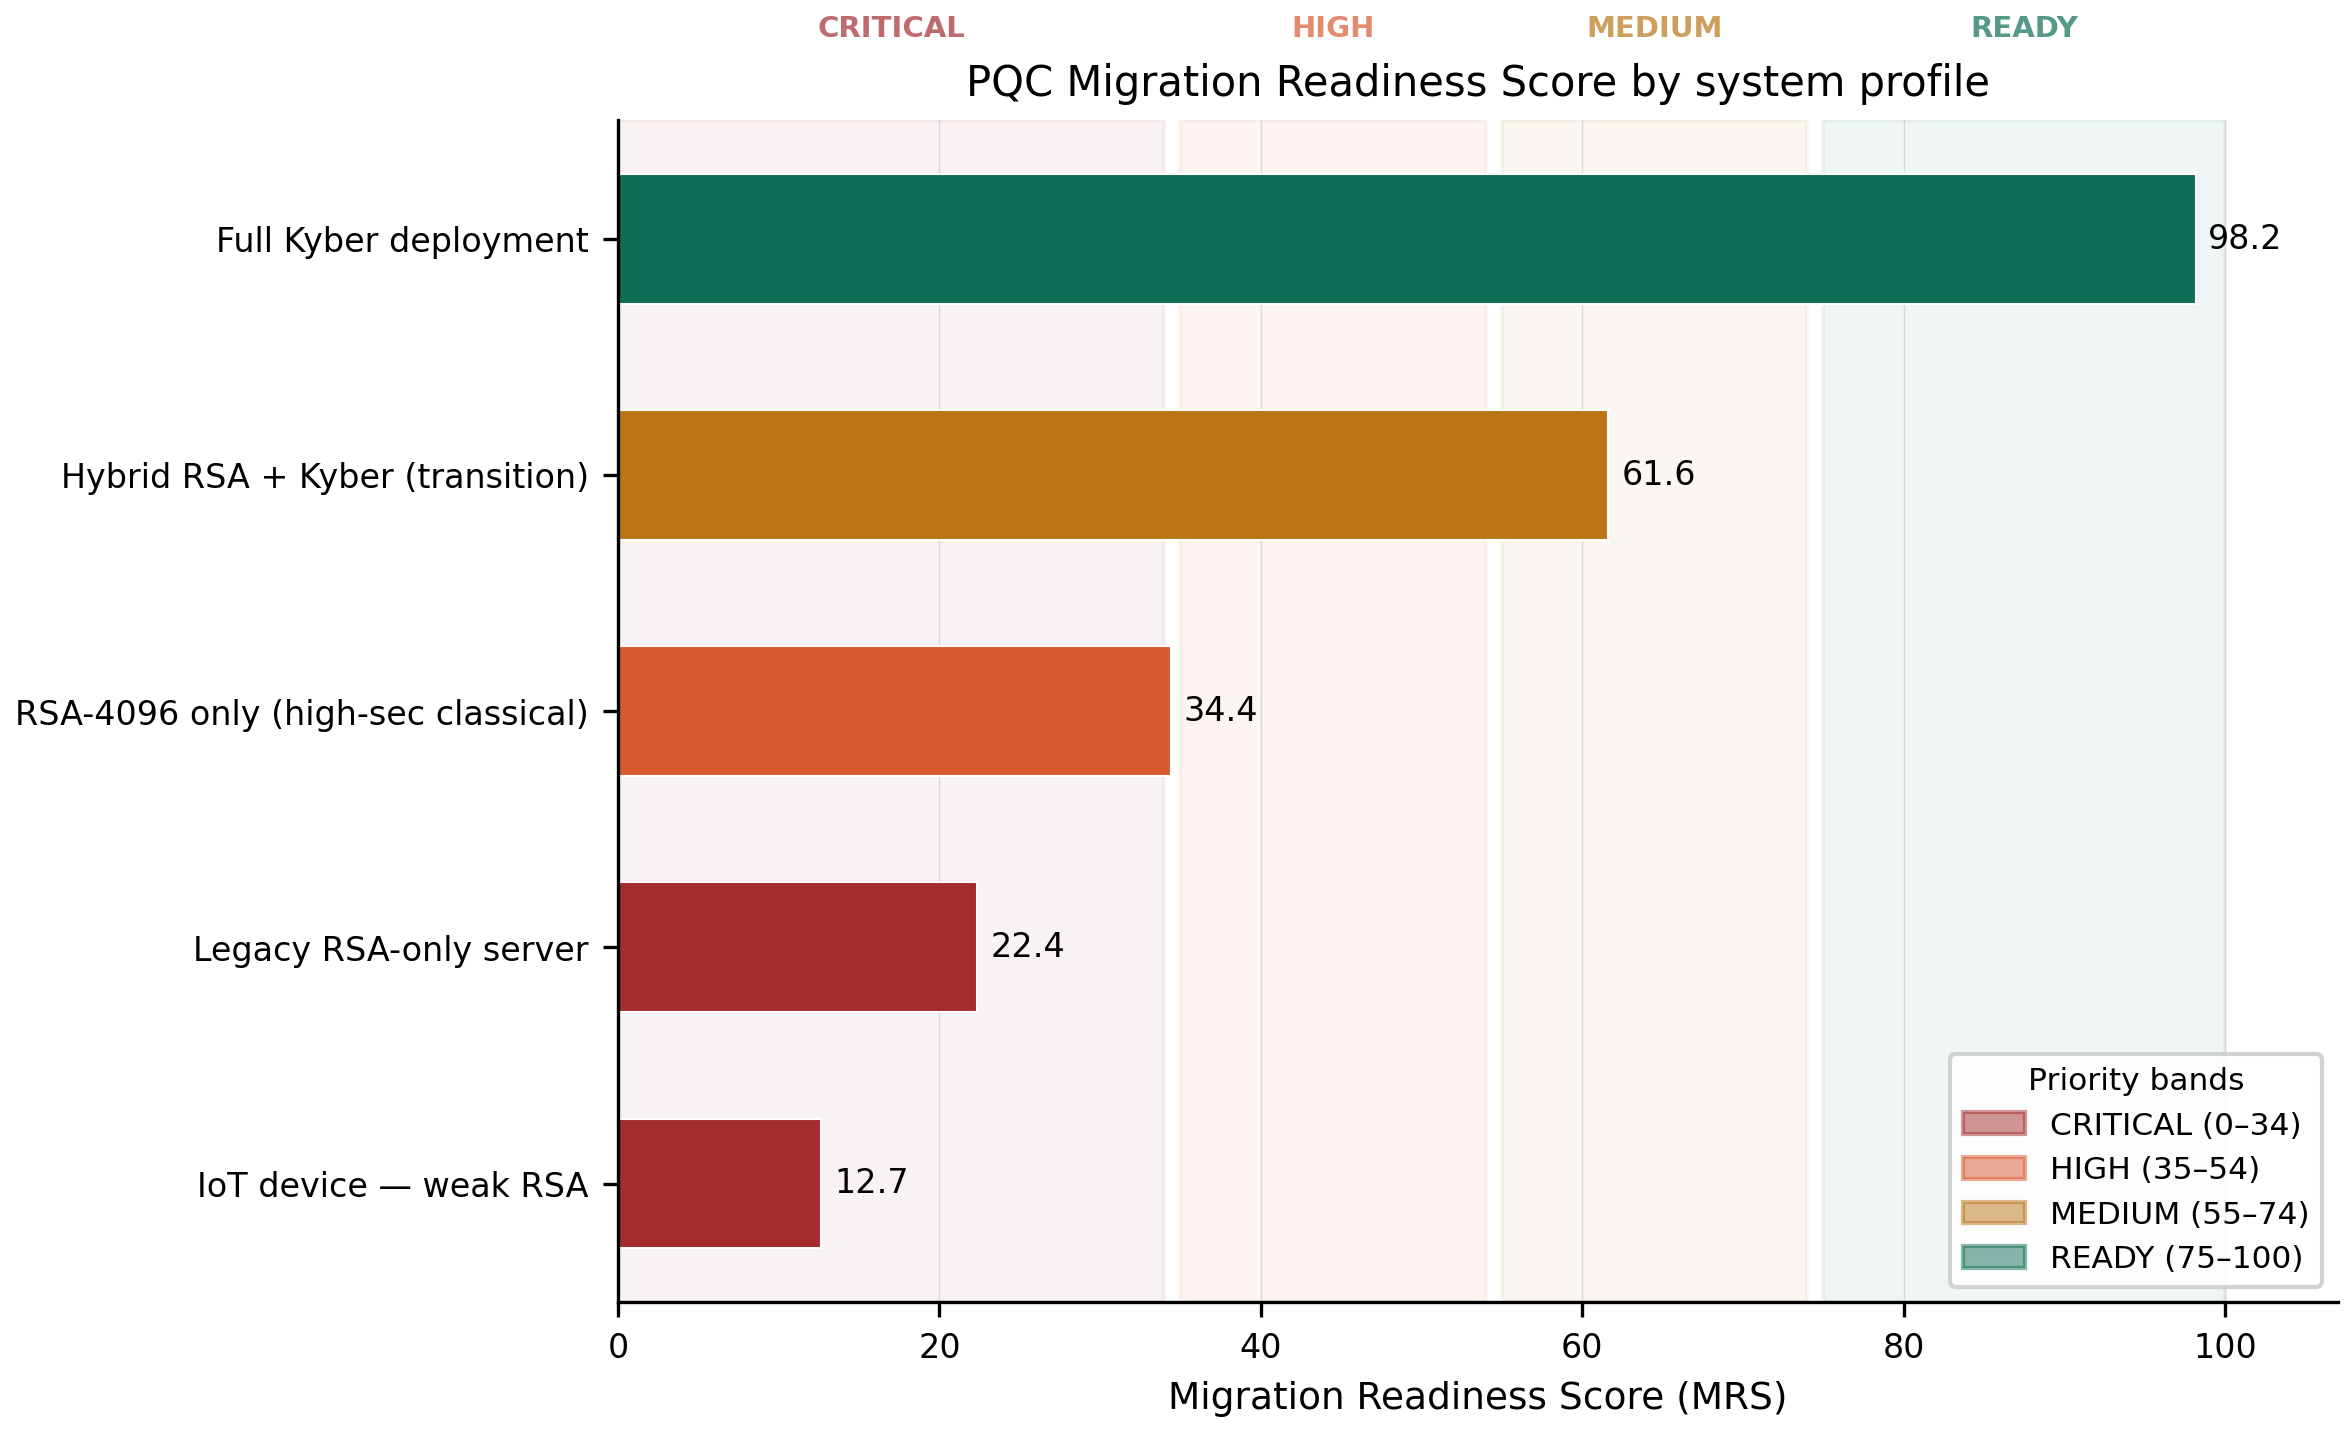
\includegraphics[width=\columnwidth]{figures/pqc_readiness_scores.png}
\caption{Post-Quantum Migration Readiness Scores (MRS) for representative deployment scenarios.}
\label{fig:mrs}
\end{figure}
In summary, the experimental results illustrate that runtime timing, CPU usage as well as memory specification give enough information for reliable and passive cryptographic fingerprinting. With the combination of multi-class classification, attacks detection, and readiness assessment toward migration, CryptoFP delivers an integrated decision-support platform to provide enterprises with cryptographic auditing assistance and migration planning in a post-quantum era.

 \section{Future Works}
Though CryptoFP shows the possibility of passive fingerprinting using runtime behavioral profiling, there are still ways to make it more scalable, applicable, and deployable.
\paragraph{Large-Scale Runtime Dataset}
The present implementation was assessed using a prototype data set acquired in a strict experimental setup. In the future, researchers seek to amplify the data set size up to over 10 800 profiling samples acquired in different hardware profiles, operating systems, and workload conditions because this would increase the robustness of the model and allow for a more thorough evaluation of deep learning architectures.
\paragraph{Support for Additional Cryptographic Algorithms}
The current structure allows for three variations of RSA and three parameter sets for ML-KEM. The upcoming release of CryptoFP will expand the support to other classical and post-quantum crypto algorithms such as ML-DSA (Dilithium), SLH-DSA (SPHINCS+), Falcon, ECC, AES, etc. This advancement will make it possible to effectively manage the cryptographic inventory in heterogeneous enterprise settings while keeping pace with the changes in post-quantum standards.
\paragraph{Advanced Machine Learning Models}
In future research, the most outstanding performance of Random Forest and SVM in the current dataset will be investigated through their operation with Transformer architectures, Graph Neural Networks (GNNs), and self-supervised representation learning. These methods are expected to yield more advanced feature representations, enhanced accuracy of classification in large datasets, and decreased need for manually produced features.
\paragraph{Enterprise Deployment and Continuous Monitoring}
The planned development of CryptoFP will transform it into a platform for monitoring cryptographic operations in real-time, tracking running applications without hampering the normal operation of the system. The combination of CryptoFP with efficiencies of enterprise Security Information and Event Management (SIEM) platforms, cloud-native monitoring solutions, and centralized logging systems will facilitate the management of cryptographic inventory and assurance of compliance of cryptographic deployments on a continuous basis in the large-scale distributed environment.

\section*{conclusion}

The paper described CryptoFP which is a passive machine learning framework that performs cryptographic algorithm fingerprinting based on run time timing, memory and processor resource utilization without the need for source-code inspection, binary code analysis and network traffic monitoring. The framework looked at six cryptographic configurations RSA-1024, RSA-2048, RSA-4096, Kyber-512, Kyber-768, Kyber-1024 and compared four machine learning methods for multiclass classification, revealing SVM as the best classification method and Random Forest as a method that produces trustworthy and understandable results.Along with algorithm identification, CryptoFP adopts a misuse detection framework and Post-Quantum Migration Readiness Score, thereby providing a unified decision-making support framework regarding cryptographic audits and migration assessments. Our findings indicate that runtime behavioral patterns are adequate for passive cryptographic fingerprinting while demonstrating the abilities of CryptoFP to help enterprises move towards NIST-standard post-quantum cryptography, which also serves to enhance benchmarking insights presented previously in our work [3].

\begin{thebibliography}{99}

\bibitem{fips203}
National Institute of Standards and Technology,
``Module-Lattice-Based Key-Encapsulation Mechanism Standard (FIPS 203),''
Federal Information Processing Standard 203, 2024.

\bibitem{kyber2021}
R. Avanzi, J. Bos, L. Ducas, E. Kiltz, T. Lepoint, V. Lyubashevsky,
J. M. Schanck, P. Schwabe, G. Seiler, and D. Stehl{\'e},
``CRYSTALS-Kyber Algorithm Specifications and Supporting Documentation,''
CRYSTALS-Kyber Team, 2021.

\bibitem{takshak2026}
T. Shetty, R. Fernandes, S. D. Salian, A. V. Singh, and A. P. Rodrigues,
``Comparative Performance and Security Evaluation of RSA and Post-Quantum Cryptography,''
in \textit{Proc. 5th Int. Conf. Innovative Practices in Technology and Management (ICIPTM)}, IEEE, 2026.

\bibitem{kocher1996}
P. C. Kocher,
``Timing Attacks on Implementations of Diffie-Hellman, RSA, DSS, and Other Systems,''
in \textit{Advances in Cryptology—CRYPTO'96},
pp. 104--113, 1996.

\bibitem{maghrebi2016}
H. Maghrebi, T. Portigliatti, and E. Prouff,
``Breaking Cryptographic Implementations Using Deep Learning Techniques,''
in \textit{Proc. Int. Conf. Security, Privacy, and Applied Cryptography Engineering (SPACE)},
pp. 3--26, 2016.

\bibitem{zhang2021}
L. Zhang and Y. Liu,
``Deep Learning-Based Side-Channel Analysis: A Survey,''
\textit{IEEE Access},
vol. 9,
pp. 12096--12115,
2021.

\bibitem{he2023}
J. He and X. Wang,
``Machine Learning Techniques for Side-Channel Cryptanalysis: A Survey,''
\textit{ACM Computing Surveys},
vol. 56,
no. 2,
2023.

\bibitem{bahdanau2015}
D. Bahdanau, K. Cho, and Y. Bengio,
``Neural Machine Translation by Jointly Learning to Align and Translate,''
in \textit{Proc. Int. Conf. Learning Representations (ICLR)},
2015.

\bibitem{sp800131a}
National Institute of Standards and Technology,
``Transitioning the Use of Cryptographic Algorithms and Key Lengths,''
NIST Special Publication 800-131A Revision 2,
2019.

\bibitem{breiman2001}
L. Breiman,
``Random Forests,''
\textit{Machine Learning},
vol. 45,
no. 1,
pp. 5--32,
2001.

\bibitem{cortes1995}
C. Cortes and V. Vapnik,
``Support-Vector Networks,''
\textit{Machine Learning},
vol. 20,
no. 3,
pp. 273--297,
1995.

\bibitem{chawla2002}
N. V. Chawla, K. W. Bowyer, L. O. Hall, and W. P. Kegelmeyer,
``SMOTE: Synthetic Minority Over-sampling Technique,''
\textit{Journal of Artificial Intelligence Research},
vol. 16,
pp. 321--357,
2002.

\bibitem{liboqs}
Open Quantum Safe Project,
``liboqs: Open Quantum Safe Project,''
2024.
Available: \url{https://openquantumsafe.org}

\end{thebibliography}
\end{document}